\documentclass[10pt,a4paper]{paper}

\usepackage[latin1]{inputenc}
\usepackage[english]{babel}

\usepackage[official,right]{eurosym}
\usepackage{hyperref}
\usepackage{graphicx}
\usepackage{a4wide}
\usepackage{calc}
%\usepackage{picins}
\usepackage{fancyhdr}
\usepackage{amssymb,amsmath}
\usepackage{gensymb}
%\usepackage{multicol}
\usepackage{url}

% For drawings
\usepackage{pgf}
\usepackage{tikz}
\usetikzlibrary{arrows,automata}
\usepackage{color}

% For quick and easy figures
\newcommand{\pic}[3]{
\begin{figure}[h]\begin{center}\includegraphics[width=#2]{#1.png} 
	\caption{#3}
	\label{#1}
\end{center}\end{figure}
}

%\newcommand{\inHfile}[2]{
%	Function \texttt{#1} in File \texttt{#2.h} \\
%}
%\newcommand{\inCfile}[2]{
%	Function \texttt{#1} in File \texttt{#2.c} \\
%}

\newcommand{\inHfile}[2]{Function \texttt{#1}\\
\indent in File \texttt{#2.h} \\}

\newcommand{\inCfile}[2]{Function \texttt{#1}\\
\indent in File \texttt{#2.c} \\}

%\numberwithin{equation}{section}
\newcommand{\vect}[1]{\ensuremath{\overrightarrow{#1}}}		%% How to mark Vectors
\newcommand{\eu}[1]{\ensuremath{#1^{\phi}}}			%% how to mark euler angles
\newcommand{\ra}[1]{\ensuremath{\omega_{#1}}}		%% how to mark rates
\newcommand{\ew}[1]{\;. \! \!#1}					%% how to mark element-wise operations
\newcommand{\mat}[1]{\ensuremath{\mathbf{#1}}}		%% how to mark Matrices
\newcommand{\eye}[0]{\mat{I}}						%% Identity matrix
\newcommand{\quat}[1]{\ensuremath{q_{#1}}}			%% how to mark Quaternions
\newcommand{\transp}[1]{\ensuremath{#1^{T}}}
\newcommand{\est}[1]{\ensuremath{\hat{#1}}}
\newcommand{\err}[1]{\ensuremath{\tilde{#1}}}
\newcommand{\meas}[1]{\ensuremath{\tilde{#1}}}
\newcommand{\linpt}[1]{\ensuremath{\overline{#1}}}
\newcommand{\norm}[1]{\ensuremath{|{#1}|}}
\newcommand{\quatprod}[0]{\ensuremath{\bullet}}
\newcommand{\ddt}[2]{\ensuremath{#1^{(#2)}}}
\newcommand{\deriv}[2]{\ensuremath{{#1}^{(#2)}}}
\newcommand{\inv}[1]{\ensuremath{#1}^{-1}}
\newcommand{\comp}[1]{\ensuremath{#1}^*}
\newcommand{\atan}[1]{\ensuremath{\text{atan}\left({#1}\right)}}
\newcommand{\sign}[1]{\ensuremath{\text{sign}\left({#1}\right)}}
\newcommand{\cross}{\ensuremath{\times}}

\newcommand{\division}[0]{\ensuremath{\div}}
\newcommand{\multiplication}[0]{\ensuremath{\cdot}}


%% Formatting in the right color for euler angles
\definecolor{rollcolor}{rgb}{0,0,1}
\definecolor{pitchcolor}{rgb}{0,0.5,0}
\definecolor{yawcolor}{rgb}{1,0,0}
\newcommand{\Rollc}[1]{\color{rollcolor}#1\color{black}{}}
\newcommand{\Pitchc}[1]{\color{pitchcolor}#1\color{black}{}}
\newcommand{\Yawc}[1]{\color{yawcolor}#1\color{black}{}}
\newcommand{\Roll}[0]{\ensuremath{\Rollc \phi}}
\newcommand{\Pitch}[0]{\ensuremath{\Pitchc \theta }}
\newcommand{\Yaw}[0]{\ensuremath{\Yawc \psi}}
\newcommand{\lon}[0]{\ensuremath{\lambda}}
\newcommand{\lat}[0]{\ensuremath{\varphi}}


\newcommand{\mynote}[1]{\begin{flushright}\fbox{Martin: ``\textit{#1}''}\end{flushright}}
%\newcommand{\mynote}[1]{}

\graphicspath{{./images/},{tmp/}}

\title{Documentation for pprz_algebra}
\author{Martin Dieblich}

\begin{document}

%\maketitle
\section{Introduction}
This is the documentation for the geodetices files of the paparazzi project (paparazzi.nongnu.org). It should be a reference for the functions which are defined in the directory \texttt{(paparazzi)/sw/airborne/math}.

\mynote{Still missing: hmsl and the gc\_of\_gd\_lat\_d conversion}
\tableofcontents
\section{ECEF}
Earth-Centered-Earth-Fixed coordinates belong to the easiest coordinates to compute, because they have a fixed frame and they don't have to regard the non-spherical shape of the earth. Though they are not intuitiv. \\
\begin{figure}[h!]
	\centering
	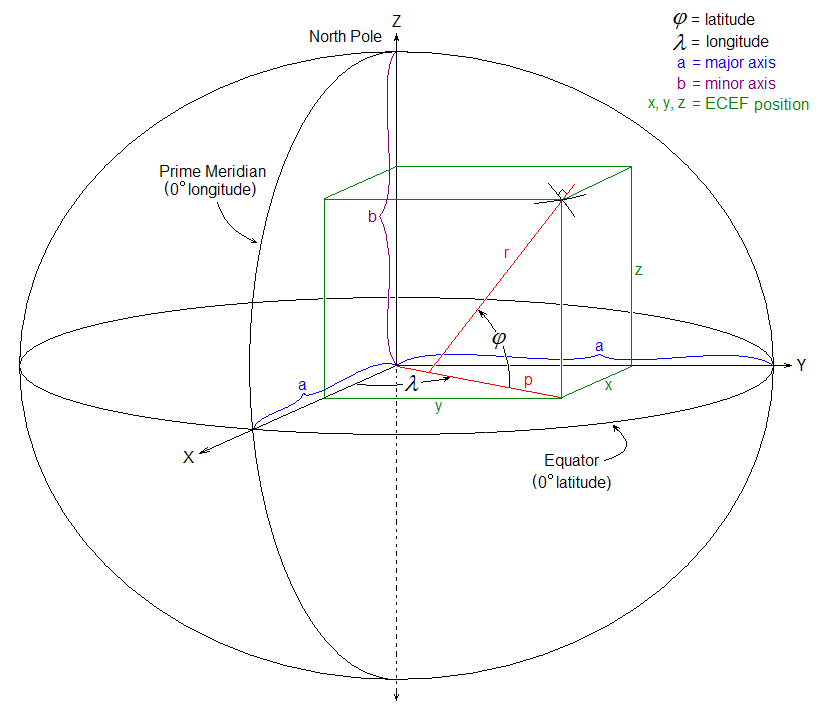
\includegraphics[width=10cm]{ECEF}
	\caption{ECEF coordinates}
	\label{ECEF coordinates}
\end{figure}

ECEF coordinates are defined using
\begin{equation}
p_{ECEF} = \begin{pmatrix} x \\ y \\ z \end{pmatrix}
\end{equation}
available for the following simple types
\begin{itemize}
\item int32\_t - \texttt{EcefCoor\_i}
\item float - \texttt{EcefCoor\_f}
\item double - \texttt{EcefCoor\_d}
\end{itemize}




\subsection{Transformations from ECEF}
\subsubsection*{to LTP}
Gets the LLA-coordinates and a transformation matrix from ECEF to ENU out of ECEF coordinates.

First, the LLA coordinates (WGS-84) are computed from the ECEF coordinates. 

With the LLA-coordinates it is possible to construct a rotational matrix.
\begin{equation}
\mat R_{ecef2enu} = \begin{pmatrix}
-\sin \lon				& \cos \lon				&		0	\\
-\sin \lat \cos \lon	& -\sin \lat \sin \lon	& \cos \lat	\\
\cos \lat \cos \lon		& \cos \lat \sin \lon	& \sin \lat	
\end{pmatrix}
\end{equation}
\inCfile{ltp\_def\_from\_ecef\_i(LtpDef\_i* def, EcefCoor\_i* ecef)}{pprz\_geodetic\_int}
\inCfile{ltp\_def\_from\_ecef\_f(LtpDef\_f* def, EcefCoor\_f* ecef)}{pprz\_geodetic\_float}
\inCfile{ltp\_def\_from\_ecef\_d(LtpDef\_d* def, EcefCoor\_d* ecef)}{pprz\_geodetic\_double}

\subsubsection*{to LLA}
Generating LLA coordinates is made using the following calculations. These refer to \cite{wiki:1} or \cite{Wendel__2007}(pages 31-33).

\begin{align}
a	&= 6,378,137										\\
f	&= \frac{1}{298.257223563}							
\end{align}
\begin{align}
b	&= a \multiplication (1-f)							\\
e^2	&= \sqrt{2f-f^2}									\\
e'	&= e \frac{a}{b}									\\
E^2	&= a^2-b^2											\\
r	&= \sqrt{ x^2 + y^2}								\\
F	&= 54 b^2 z^2										\\
G	&= r^2 + (1-e^2)z^2-e^2E^2							\\
c	&= \frac{e^4Fr^2}{G^3}								\\
s	&= \sqrt[3]{1+c+\sqrt{c^2+2c}}						\\
P	&= \frac{F}{3\left(s+\tfrac 1 s + 1\right)^2 G^2}	\\
Q	&= \sqrt{1+2e^4P}									\\
r_0	&= -\frac{Pe^2r}{1+Q} + \sqrt{\tfrac 1 2 a^2 \left(1 + \tfrac 1 Q \right) - \frac{P(1-e^2)z^2}{Q(1+Q)}-\tfrac 1 2 P r^2}	\\
U	&= \sqrt{(r-e^2r_0)^2+z^2}							\\
V	&= \sqrt{(r-e^2r_0)^2+(1-e^2)z^2}					\\
z_0	&= \frac{b^2z}{aV}									\\
\lat	&= \arctan \left( \frac{z+(e')^2z_0} r \right)	\\
\lon	&= atan2(y,x)									\\
h	&= U \left( \frac{b^2}{aV} - 1 \right)
\end{align}
\inCfile{lla\_of\_ecef\_i(LlaCoor\_i* out, EcefCoor\_i* in)}{pprz\_geodetic\_int}
\inCfile{lla\_of\_ecef\_f(LlaCoor\_f* out, EcefCoor\_f* in)}{pprz\_geodetic\_float}
\inCfile{lla\_of\_ecef\_d(LlaCoor\_d* lla, EcefCoor\_d* ecef)}{pprz\_geodetic\_double}

\subsubsection*{to NED/ENU}
With a know transformation matrix (see section \ref{LTP}) it is quite easy to rotate a vector into the ENU frame:
\begin{equation}
\vect v_{ENU} = \mat R_{ecef2enu} \vect v_{ECEF}
\end{equation}
For a transformation into the NED-frame you have to do an additional ENU/NED-transformation.

\inCfile{enu\_of\_ecef\_vect\_i(EnuCoor\_i* enu, LtpDef\_i* def, EcefCoor\_i* ecef)}{pprz\_geodetic\_int}
\inCfile{ned\_of\_ecef\_vect\_i(NedCoor\_i* ned, LtpDef\_i* def, EcefCoor\_i* ecef)}{pprz\_geodetic\_int}
\inCfile{enu\_of\_ecef\_vect\_f(EnuCoor\_f* enu, LtpDef\_f* def, EcefCoor\_f* ecef)}{pprz\_geodetic\_float}
\inCfile{ned\_of\_ecef\_vect\_f(NedCoor\_f* ned, LtpDef\_f* def, EcefCoor\_f* ecef)}{pprz\_geodetic\_float}
\inCfile{enu\_of\_ecef\_vect\_d(EnuCoor\_d* enu, LtpDef\_d* def, EcefCoor\_d* ecef)}{pprz\_geodetic\_double}
\inCfile{ned\_of\_ecef\_vect\_d(NedCoor\_d* ned, LtpDef\_d* def, EcefCoor\_d* ecef)}{pprz\_geodetic\_double}

The transformation of a point is very similiar. Instead of a point you use a difference vector between the desired point $p_d$ and the center of the local tangent plane $p_0$.
\begin{equation}
\vect v_{ECEF} = p_d - p_0
\end{equation}
\inCfile{enu\_of\_ecef\_point\_i(EnuCoor\_i* enu, LtpDef\_i* def, EcefCoor\_i* ecef)}{pprz\_geodetic\_int}
\inCfile{ned\_of\_ecef\_point\_i(NedCoor\_i* ned, LtpDef\_i* def, EcefCoor\_i* ecef)}{pprz\_geodetic\_int}
\inCfile{enu\_of\_ecef\_point\_f(EnuCoor\_f* enu, LtpDef\_f* def, EcefCoor\_f* ecef)}{pprz\_geodetic\_float}
\inCfile{ned\_of\_ecef\_point\_f(NedCoor\_f* ned, LtpDef\_f* def, EcefCoor\_f* ecef)}{pprz\_geodetic\_float}
\inCfile{enu\_of\_ecef\_point\_d(EnuCoor\_d* enu, LtpDef\_d* def, EcefCoor\_d* ecef)}{pprz\_geodetic\_double}
\inCfile{ned\_of\_ecef\_point\_d(NedCoor\_d* ned, LtpDef\_d* def, EcefCoor\_d* ecef)}{pprz\_geodetic\_double}


\subsection{Transformations to ECEF}
\subsubsection*{from LLA}
Calculating the ECEF coordinates out of LLA coordinates is a slightly easier task than the other way round. The following way refers to \cite{wiki:1}. With the known constants
\begin{align}
a	&= 6,378,137				\\
f	&= \frac{1}{298.257223563}	\\
e^2	&= \sqrt{2f-f^2}			
\end{align}
the value
\begin{equation}
\chi = \sqrt{1-e^2\sin^2 \lat}
\end{equation}
can be precomputed and used in
\begin{align}
x &= \left(\tfrac a \chi + h \right) \cos \lat \cos \lon \\
y &= \left(\tfrac a \chi + h \right) \cos \lat \sin \lon \\
z &= \left(\tfrac a \chi (1-e^2) + h \right) \sin \lat
\end{align}
\inCfile{ecef\_of\_lla\_i(EcefCoor\_i* out, LlaCoor\_i* in)}{pprz\_geodetic\_int}
\inCfile{ecef\_of\_lla\_f(EcefCoor\_f* out, LlaCoor\_f* in)}{pprz\_geodetic\_float}
\inCfile{ecef\_of\_lla\_d(EcefCoor\_d* ecef, LlaCoor\_d* lla)}{pprz\_geodetic\_double}

\subsubsection*{from NED/ENU}
With a know transformation matrix (see section \ref{LTP}) it is quite easy to rotate a vector from the ENU-frame to the ECEF-frame.
Since
\begin{equation}
\mat R_{enu2ecef} = \inv{\mat R_{ecef2enu}} = \transp{\mat R_{ecef2enu}}
\end{equation}
a transformation is done as follows
\begin{equation}
\vect v_{ECEF} = \mat R_{enu2ecef} \vect v_{ENU} 
\end{equation}
For a transformation from the NED-frame you have to do an additional ENU/NED-transformation before.

\inCfile{ecef\_of\_enu\_vect\_d(EcefCoor\_d* ecef, LtpDef\_d* def, EnuCoor\_d* enu)}{pprz\_geodetic\_double}
\inCfile{ecef\_of\_ned\_vect\_d(EcefCoor\_d* ecef, LtpDef\_d* def, NedCoor\_d* ned)}{pprz\_geodetic\_double}

The transformation of a point is very similiar. After transforming into the ECEF-frame you add the position of the center  $p_0$ to the result.
\begin{equation}
\vect p_{ECEF} = p + p_0
\end{equation}
\inCfile{ecef\_of\_enu\_point\_d(EcefCoor\_d* ecef, LtpDef\_d* def, EnuCoor\_d* enu)}{pprz\_geodetic\_double}
\inCfile{ecef\_of\_ned\_point\_d(EcefCoor\_d* ecef, LtpDef\_d* def, NedCoor\_d* ned)}{pprz\_geodetic\_double}

\section{LLA}
LLA coordinates (longitude, lattitude, attitude) are the more intuitive way to express a position on the earth's surface. The values ``longitude'' and ``lattitude'' are angles and therefore in degrees or radians and the ``attitude'' is in meters above the surface of the earth's approximated shape. 

\begin{figure}[h!]
	\centering
	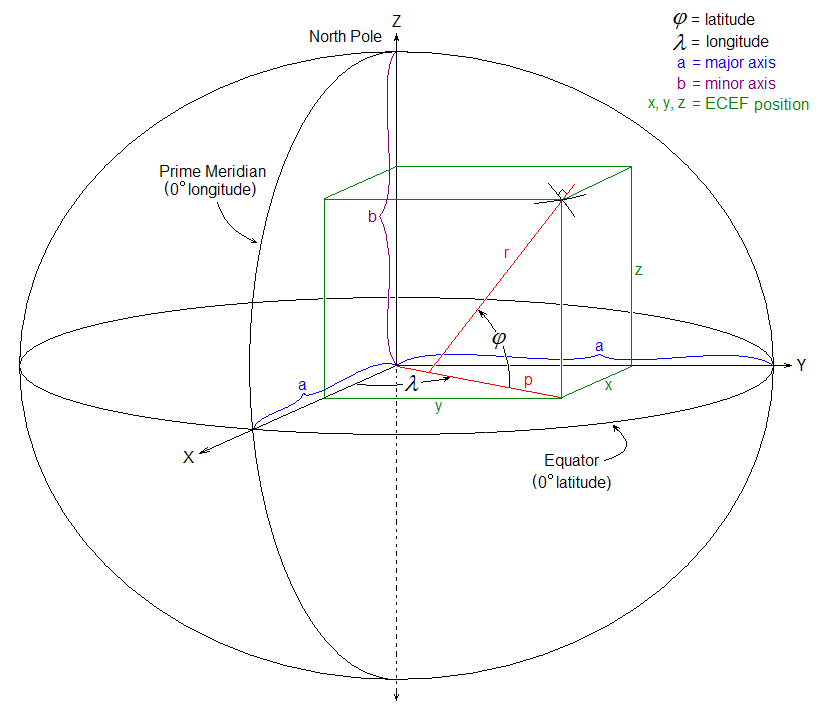
\includegraphics[width=10cm]{ECEF}
	\caption{LLA coordinates}
	\label{LLA coordinates1}
\end{figure}

LLA coordinates are defined using
\begin{equation}
p_{LLA} = \begin{pmatrix} \lat \\ \lon \\ h \end{pmatrix}
\end{equation}
available for the following simple types
\begin{itemize}
\item int32\_t - \texttt{LlaCoor\_i}
\item float - \texttt{LlaCoor\_f}
\item double - \texttt{LlaCoor\_d}
\end{itemize}

\subsection{Simple Operations}
\subsubsection*{Assigning}
It is either possible to assign every single value of LLA-coordinate
\begin{equation}
pos = \begin{pmatrix}	\lat	\\
						\lon	\\
						h		\end{pmatrix}
\end{equation}
\inHfile{LLA\_ASSIGN(pos, lat, lon, alt)}{pprz\_geodetic}

\noindent
or to copy one coordinate to another

\texttt{pos1 = pos2}\\
\inHfile{LLA\_COPY(pos1, pos2)}{pprz\_geodetic}


\subsection{Trasnformation from LLA}
\subsubsection*{to ECEF}
Calculating the ECEF coordinates out of LLA coordinates is a slightly easier task than the other way round. The following way refers to \cite{wiki:1}. With the known constants
\begin{align}
a	&= 6,378,137				\\
f	&= \frac{1}{298.257223563}	\\
e^2	&= \sqrt{2f-f^2}			
\end{align}
the value
\begin{equation}
\chi = \sqrt{1-e^2\sin^2 \lat}
\end{equation}
can be precomputed and used in
\begin{align}
x &= \left(\tfrac a \chi + h \right) \cos \lat \cos \lon \\
y &= \left(\tfrac a \chi + h \right) \cos \lat \sin \lon \\
z &= \left(\tfrac a \chi (1-e^2) + h \right) \sin \lat
\end{align}
\inCfile{ecef\_of\_lla\_i(EcefCoor\_i* out, LlaCoor\_i* in)}{pprz\_geodetic\_int}
\inCfile{ecef\_of\_lla\_f(EcefCoor\_f* out, LlaCoor\_f* in)}{pprz\_geodetic\_float}
\inCfile{ecef\_of\_lla\_d(EcefCoor\_d* ecef, LlaCoor\_d* lla)}{pprz\_geodetic\_double}


\subsection{Transforming to LLA}
\subsubsection*{from ECEF}
Generating LLA coordinates is made using the following calculations. These refer to \cite{wiki:1} or \cite{Wendel__2007}(pages 31-33).

\begin{align}
a	&= 6,378,137										\\
f	&= \frac{1}{298.257223563}							
\end{align}
\begin{align}
b	&= a \multiplication (1-f)							\\
e^2	&= \sqrt{2f-f^2}									\\
e'	&= e \frac{a}{b}									\\
E^2	&= a^2-b^2											\\
r	&= \sqrt{ x^2 + y^2}								\\
F	&= 54 b^2 z^2										\\
G	&= r^2 + (1-e^2)z^2-e^2E^2							\\
c	&= \frac{e^4Fr^2}{G^3}								\\
s	&= \sqrt[3]{1+c+\sqrt{c^2+2c}}						\\
P	&= \frac{F}{3\left(s+\tfrac 1 s + 1\right)^2 G^2}	\\
Q	&= \sqrt{1+2e^4P}									\\
r_0	&= -\frac{Pe^2r}{1+Q} + \sqrt{\tfrac 1 2 a^2 \left(1 + \tfrac 1 Q \right) - \frac{P(1-e^2)z^2}{Q(1+Q)}-\tfrac 1 2 P r^2}	\\
U	&= \sqrt{(r-e^2r_0)^2+z^2}							\\
V	&= \sqrt{(r-e^2r_0)^2+(1-e^2)z^2}					\\
z_0	&= \frac{b^2z}{aV}									\\
\lat	&= \arctan \left( \frac{z+(e')^2z_0} r \right)	\\
\lon	&= atan2(y,x)									\\
h	&= U \left( \frac{b^2}{aV} - 1 \right)
\end{align}
\inCfile{lla\_of\_ecef\_i(LlaCoor\_i* out, EcefCoor\_i* in)}{pprz\_geodetic\_int}
\inCfile{lla\_of\_ecef\_f(LlaCoor\_f* out, EcefCoor\_f* in)}{pprz\_geodetic\_float}
\inCfile{lla\_of\_ecef\_d(LlaCoor\_d* lla, EcefCoor\_d* ecef)}{pprz\_geodetic\_double}
\section{LTP}\label{LTP}
The Local Tangent Plane (LTP) is an approximation of the earth at a fixed position. It is defined using an ECEF position, a LLA position and a rotational matrix to convert between them. \emph{Please note that the matrix transforms from ECEF to ENU!}
\begin{verbatim}
LtpDef   = {      ecef      lla      ltp_of_ecef     }
\end{verbatim}
It is available for the following simple types:\\
\begin{tabular}{c|cccc}
sinmple type & struct name & $p_{ECEF}$ & $p_{LLA}$ & $\mat R_{ltp\_of\_ecef}$\\  \hline 
int32\_t & LtpDef\_i & EcefCoor\_i  ecef & LlaCoor\_i   lla & INT32Mat33 ltp\_of\_ecef\\
float & LtpDef\_f & EcefCoor\_f  ecef & LlaCoor\_f   lla & FloatMat33 ltp\_of\_ecef\\
double & LtpDef\_d & EcefCoor\_d  ecef & LlaCoor\_d   lla & DoubleMat33 ltp\_of\_ecef 
\end{tabular} 
The fixed-point struct has hmsl (height above mean sea level) as an additional parameter.

\subsection{Transformations to LTP}
\subsubsection*{from ECEF}
Gets the LLA-coordinates and a transformation matrix from ECEF to ENU out of ECEF coordinates.

First, the LLA coordinates (WGS-84) are computed from the ECEF coordinates. 

With the LLA-coordinates it is possible to construct a rotational matrix.
\begin{equation}
\mat R_{ecef2enu} = \begin{pmatrix}
-\sin \lon				& \cos \lon				&		0	\\
-\sin \lat \cos \lon	& -\sin \lat \sin \lon	& \cos \lat	\\
\cos \lat \cos \lon		& \cos \lat \sin \lon	& \sin \lat	
\end{pmatrix}
\end{equation}
\inCfile{ltp\_def\_from\_ecef\_i(LtpDef\_i* def, EcefCoor\_i* ecef)}{pprz\_geodetic\_int}
\inCfile{ltp\_def\_from\_ecef\_f(LtpDef\_f* def, EcefCoor\_f* ecef)}{pprz\_geodetic\_float}
\inCfile{ltp\_def\_from\_ecef\_d(LtpDef\_d* def, EcefCoor\_d* ecef)}{pprz\_geodetic\_double}
\section{NED / ENU}
North-East-Down or East-North-Up coordinates are fixed in the local tangent plane. 

NED and ENU coordinates are defined using
\begin{equation}
p_{NED} = \begin{pmatrix} x \\ y \\ z \end{pmatrix} \qquad
p_{ENU} = \begin{pmatrix} x \\ y \\ z \end{pmatrix}
\end{equation}
available for the following simple types
\begin{itemize}
\item int32\_t - \texttt{NedCoor\_i} and \texttt{EnuCoor\_i}
\item float - \texttt{NedCoor\_f} and \texttt{EnuCoor\_f}
\item double - \texttt{NedCoor\_d} and \texttt{EnuCoor\_d}
\end{itemize}

\subsection{Transformation between NED and ENU}
The transformation between NED and ENU is rather simple. It can be expressed using a rotational matrix:
\begin{equation}
p_{NED} = \begin{pmatrix}
0 & 1 &  0 \\
1 & 0 &  0 \\
0 & 0 & -1
\end{pmatrix}
p_{ENU} \qquad p_{ENU} = \begin{pmatrix}
0 & 1 &  0 \\
1 & 0 &  0 \\
0 & 0 & -1
\end{pmatrix} p_{NED}
\end{equation}
or directly switching the values
\begin{equation}
\begin{pmatrix}x \\ y \\  z \end{pmatrix}_{NED} = 
\begin{pmatrix}y \\ x \\ -z \end{pmatrix}_{ENU}
\end{equation}
\inHfile{ENU\_OF\_TO\_NED(po, pi)}{pprz\_geodetic}
\inHfile{INT32\_VECT2\_ENU\_OF\_NED(o, i)}{pprz\_geodetic\_int}
\inHfile{INT32\_VECT2\_NED\_OF\_ENU(o, i)}{pprz\_geodetic\_int}
\inHfile{INT32\_VECT3\_ENU\_OF\_NED(o, i)}{pprz\_geodetic\_int}
\inHfile{INT32\_VECT3\_NED\_OF\_ENU(o, i)}{pprz\_geodetic\_int}



\subsection{Transformation from NED/ENU}
\subsubsection*{to ECEF}
With a know transformation matrix (see section \ref{LTP}) it is quite easy to rotate a vector from the ENU-frame to the ECEF-frame.
Since
\begin{equation}
\mat R_{enu2ecef} = \inv{\mat R_{ecef2enu}} = \transp{\mat R_{ecef2enu}}
\end{equation}
a transformation is done as follows
\begin{equation}
\vect v_{ECEF} = \mat R_{enu2ecef} \vect v_{ENU} 
\end{equation}
For a transformation from the NED-frame you have to do an additional ENU/NED-transformation before.

\inCfile{ecef\_of\_enu\_vect\_d(EcefCoor\_d* ecef, LtpDef\_d* def, EnuCoor\_d* enu)}{pprz\_geodetic\_double}
\inCfile{ecef\_of\_ned\_vect\_d(EcefCoor\_d* ecef, LtpDef\_d* def, NedCoor\_d* ned)}{pprz\_geodetic\_double}

The transformation of a point is very similiar. After transforming into the ECEF-frame you add the position of the center  $p_0$ to the result.
\begin{equation}
\vect p_{ECEF} = p + p_0
\end{equation}
\inCfile{ecef\_of\_enu\_point\_d(EcefCoor\_d* ecef, LtpDef\_d* def, EnuCoor\_d* enu)}{pprz\_geodetic\_double}
\inCfile{ecef\_of\_ned\_point\_d(EcefCoor\_d* ecef, LtpDef\_d* def, NedCoor\_d* ned)}{pprz\_geodetic\_double}


\subsection{Transformation to NED/ENU}
\subsubsection*{from ECEF}
With a know transformation matrix (see section \ref{LTP}) it is quite easy to rotate a vector into the ENU frame:
\begin{equation}
\vect v_{ENU} = \mat R_{ecef2enu} \vect v_{ECEF}
\end{equation}
For a transformation into the NED-frame you have to do an additional ENU/NED-transformation.

\inCfile{enu\_of\_ecef\_vect\_i(EnuCoor\_i* enu, LtpDef\_i* def, EcefCoor\_i* ecef)}{pprz\_geodetic\_int}
\inCfile{ned\_of\_ecef\_vect\_i(NedCoor\_i* ned, LtpDef\_i* def, EcefCoor\_i* ecef)}{pprz\_geodetic\_int}
\inCfile{enu\_of\_ecef\_vect\_f(EnuCoor\_f* enu, LtpDef\_f* def, EcefCoor\_f* ecef)}{pprz\_geodetic\_float}
\inCfile{ned\_of\_ecef\_vect\_f(NedCoor\_f* ned, LtpDef\_f* def, EcefCoor\_f* ecef)}{pprz\_geodetic\_float}
\inCfile{enu\_of\_ecef\_vect\_d(EnuCoor\_d* enu, LtpDef\_d* def, EcefCoor\_d* ecef)}{pprz\_geodetic\_double}
\inCfile{ned\_of\_ecef\_vect\_d(NedCoor\_d* ned, LtpDef\_d* def, EcefCoor\_d* ecef)}{pprz\_geodetic\_double}

The transformation of a point is very similiar. Instead of a point you use a difference vector between the desired point $p_d$ and the center of the local tangent plane $p_0$.
\begin{equation}
\vect v_{ECEF} = p_d - p_0
\end{equation}
\inCfile{enu\_of\_ecef\_point\_i(EnuCoor\_i* enu, LtpDef\_i* def, EcefCoor\_i* ecef)}{pprz\_geodetic\_int}
\inCfile{ned\_of\_ecef\_point\_i(NedCoor\_i* ned, LtpDef\_i* def, EcefCoor\_i* ecef)}{pprz\_geodetic\_int}
\inCfile{enu\_of\_ecef\_point\_f(EnuCoor\_f* enu, LtpDef\_f* def, EcefCoor\_f* ecef)}{pprz\_geodetic\_float}
\inCfile{ned\_of\_ecef\_point\_f(NedCoor\_f* ned, LtpDef\_f* def, EcefCoor\_f* ecef)}{pprz\_geodetic\_float}
\inCfile{enu\_of\_ecef\_point\_d(EnuCoor\_d* enu, LtpDef\_d* def, EcefCoor\_d* ecef)}{pprz\_geodetic\_double}
\inCfile{ned\_of\_ecef\_point\_d(NedCoor\_d* ned, LtpDef\_d* def, EcefCoor\_d* ecef)}{pprz\_geodetic\_double}

\subsubsection*{from LLA}
This functions transforms a point from the LLA coordinates in the ECEF-frame and then into the NED-/ENU-frame.
\inCfile{enu\_of\_lla\_point\_i(EnuCoor\_i* enu, LtpDef\_i* def, LlaCoor\_i* lla)}{pprz\_geodetic\_int}
\inCfile{ned\_of\_lla\_point\_i(NedCoor\_i* ned, LtpDef\_i* def, LlaCoor\_i* lla)}{pprz\_geodetic\_int}

\bibliographystyle{acm} 
\bibliography{headfile}
%
\end{document}